%%%%%%%%%%%%%%%%%%%%%%%%%%%%%%%%%%%%%%%%%%%%%%%%%%%%%%%%%%%%%%%%%%%%%%%%%%%%%%%%
%%
%% CT Lab Notes
%% Copyright (C) 2017  Joshua Ellis
%% Department of Physics
%% The University of Melbourne
%%
%%%%%%%%%%%%%%%%%%%%%%%%%%%%%%%%%%%%%%%%%%%%%%%%%%%%%%%%%%%%%%%%%%%%%%%%%%%%%%%%

%%%%%%%%%%%%%%%%%%%%%%%%%%%%%%%%%%%%%%%%%%%%%%%%%%%%%%%%%%%%%%%%%%%%%%%%%%%%%%%%
%% HEADER
%%%%%%%%%%%%%%%%%%%%%%%%%%%%%%%%%%%%%%%%%%%%%%%%%%%%%%%%%%%%%%%%%%%%%%%%%%%%%%%%

%% In general, LaTeX commands start with `\` and consist of letters only.
%% Optional parameters are specified in brackets `[]`, whilst compulsory
%% arguments (if any) are specified in braces `{}`.  (Strictly speaking, this is
%% only a convention and packages can use other things.  One notable example is
%% the Beamer package which adds extra optional arguments with `<>'.)
%%
%% LaTeX is generally insensitive to whitespaces including newlines.  So if a
%% functions takes a lot of arguments or has many options, it can be easily
%% split across lines without repercussions.  The one important exception is
%% that full empty lines mark the end/start of a paragraph.

%% All LaTeX documents begin with the the `\documentclass` command which serves
%% to set the general style of the document.  It defines the page layout, the
%% chapter/section styles, how figures appear, etc. and may provide some
%% additional environments too.  LaTeX comes with four main classes: `article`,
%% `report`, `book` and `letter`.
%%
%% The [KOMA-script](https://www.ctan.org/pkg/koma-script) package provides
%% alternatives to replacements for the default classes (`scrartcl`, `scrreprt`,
%% `scrbook`, `scrlttr2`) and provides a lot of options to more easily customize the
%% layout of the page.
\documentclass[
  a4paper,             % The size of the layout
  11pt,                % The font size (10pt, 11pt, 12pt)
  oneside,             % Whether the document is one-sided or two-sided
  onecolumn,           % Whether to have one or two columns in the layout
  bibliography=totoc,  % Adjust how the bibliography appears in ToC
  final,               % As opposed to draft (which speeds up compilation)
]{scrartcl}
%% Note all of these optional arguments are required; in fact, most of the ones
%% specified here would have been chosen by default if left unspecified.  There
%% are also some other options which have not be specified but they are
%% documented in the [KOMA-script](https://www.ctan.org/pkg/koma-script)
%% documentation.
%%
%% One of the important options in the list above is `draft`/`final`.  If draft
%% mode is enabled, LaTeX and most packages will disable features which take up
%% a lot of time in order to speed up compilation.  Draft mode also highlights
%% certain error in the output document.  On the other hand, final mode enables
%% all features which will increase (sometimes quite significantly) the
%% compilation time of the document.

%% The part of the document starting from here through to the `\begin{document}`
%% command is called the preamble.  This is where you include additional
%% packages which provide additional functionalities.  Below are many packages
%% which I use on a semi-regular basis.
%%
%% Although you'll find that they are all enabled below, this is for the sake of
%% checking compatibility between all the packages.  It is advisable to only
%% enable those packages you actually need as this will speed up compilation,
%% and decrease the likelihood that two packages conflict.
%%
%% All packages are available from the Comprehence TeX Archive Network (CTAN) at
%% http://ctan.org.  Quite often, for each `\usepackage{pkg-name}`, it is
%% possible to go to http://ctan.org/pkg/pkg-name in order to find information
%% about the package (there are a few exception to this though, in which case a
%% Google search will suffice).
%%
%% Although you'll know the reason for including a package initially, most
%% people will forget this initial reason after a few months.  It is a **VERY**
%% good idea to have a small comment next to *EVERY* `\usepackage` giving a
%% quick recap as to what this package does.  This will be invaluable in case
%% you include two packages which conflict each other.

%% For the vast majority of packages, the order in which they are loaded does
%% not matter.  There are a few exceptions though, mostly relating to the
%% various referencing packages (hyperef, cleveref, ...).  The following package
%% must be loaded first and provides some additional functionalities to other
%% packages.
\usepackage{ifluatex}  % Provides the command \ifluatex

%% Formatting
%%%%%%%%%%%%%%%%%%%%%%%%%%%%%%%%%%%%%%%%%%%%%%%%%%%%%%%%%%%%%%%%%%%%%%%%%%%%%%%%

\usepackage{geometry}   % Customize text width, page height, margins, etc.
\geometry{
  %% See the geometry package's documentation for all the options available
  textwidth=13cm,
}

\usepackage{pageslts}   % Improved page numbering
\usepackage{enumitem}   % Easily customize lists

%% Change the formatting of titles and sections.
\setkomafont{part}{\normalfont\scshape\Huge}
\setkomafont{partnumber}{\normalfont\scshape\huge}
\setkomafont{section}{\normalfont\Huge}
\setkomafont{subsection}{\normalfont\huge}
\setkomafont{subsubsection}{\normalfont\Large}
\setkomafont{paragraph}{\normalfont\large\scshape}

%% Change the formatting of section entries in the table of contents
\setkomafont{sectionentry}{\scshape}

%% Modify the indentation at the start of each paragraph.
\setlength\parindent{1em}
\setlength\parskip{0.3\baselineskip plus 0.5\baselineskip minus 0.1\baselineskip}

%% Font
%%%%%%%%%%%%%%%%%%%%%%%%%%%%%%%%%%%%%%%%%%%%%%%%%%%%%%%%%%%%%%%%%%%%%%%%%%%%%%%%

\usepackage{microtype}   % Fine small typographical details
\usepackage{realscripts} % Use the font's sub- and superscripts

%% LaTeX allows for some if-else statements.  It is very rare that you'll have
%% to use them, though this is one example since we only want to include a
%% particular package if this example is compiled with LuaLaTeX.
\ifluatex
  \usepackage{fontspec}  % Allows for any font to be specified

  % Change the main font
  \setmainfont{EB Garamond}[
    Contextuals={Alternate},
    Ligatures={Common,Contextual,Rare,TeX},
    Numbers=OldStyle,
    % CharacterVariant={1},    % historical s
    % CharacterVariant={3},    % historical j
    % CharacterVariant={6},    % guillemets
    % CharacterVariant={11},   % distinguish i and 1
    % CharacterVariant={21},   % a
    % CharacterVariant={27},   % g
    ItalicFeatures={
      CharacterVariant={4},  % &
      CharacterVariant={5:3},  % v
    }
  ]

  % Change the mono-space font
  \setmonofont{Fira Code}[
    Scale=MatchLowercase,
  ]
\else
  \usepackage{ebgaramond}  % A fall-back that isn't as nice as fontspec
\fi %% marks the end of the if-else statement

\usepackage[cmintegrals,varg]{newtxmath}  % Nice math font with Garamond

%% Languages
%%%%%%%%%%%%%%%%%%%%%%%%%%%%%%%%%%%%%%%%%%%%%%%%%%%%%%%%%%%%%%%%%%%%%%%%%%%%%%%%

\usepackage[UKenglish]{babel}           % Set up the language
\usepackage[style=british]{csquotes}    % Advanced handling of quotes
\usepackage[perpage]{footmisc}          % Count per-page

%% siunitx is an incredible useful package to display numbers and their
%% associated units.  It also offers extra commands to specify lists and ranges
%% of values with units.  Some commands which it provides include:
%% - \SI{quantity}{units}
%% - \SIRange{start}{end}{units}
%% - \SIList{a, b, ..., d}{units}
%% With the units being given as `\kilo\metre\per\year\per\pico\barn`.
\usepackage{siunitx}

%% Adjust the way units are displayed in ranges and units so that they are only
%% mentinoed once.
\sisetup{
  range-units=single,
  list-units=single,
}

%% Graphics & Figure
%%%%%%%%%%%%%%%%%%%%%%%%%%%%%%%%%%%%%%%%%%%%%%%%%%%%%%%%%%%%%%%%%%%%%%%%%%%%%%%%

%% Graphics can be included in a LaTeX document with
%%
%% ```
%% \includegraphics[options]{image}
%% ```
%%
%% Usually, the extension for the image is not specified and LaTeX will
%% figure out the best one.  It is of course possible to add the extension to
%% specify a particular image.
%%
%% In order to ensure that the image is a particular width, you can use
%% `width=<distance>`.  This will also scale the height but keep the aspect
%% ratio (if you also specify the height, the aspect ratio will not be kept).
%% It is tempting to specify an exact distance such as `4cm`; but it is
%% generally better to have a relative distance such as `0.4\linewidth`.  This
%% way, the image will scale nicely if the context is changed.
\usepackage{graphicx}   % Handle graphics

%% Look for images in the './images/' sub-directory
\graphicspath{{./images/}}

\usepackage{xcolor}     % Define and use colours
\usepackage{subcaption} % Subfigures inside a figure

\usepackage{tikz}       % Powerful drawing language
\usepackage{pgfplots}   % Plotting with LaTeX
\usepackage{pgfplotstable}
\pgfplotsset{compat=1.15}

\input{pgfplots.default.tex}

\usetikzlibrary{
  matrix,
}

%% Taken from:
%% https://tex.stackexchange.com/a/83865/26980
%% Usage: 'color cells={min=..., max=...}
\usepackage{colortbl}
\pgfplotstableset{
  /color cells/min/.initial=0,
  /color cells/max/.initial=4,
  /color cells/textcolor/.initial=,
  color cells/.code={%
    \pgfqkeys{/color cells}{#1}%
    \pgfkeysalso{%
      postproc cell content/.code={%
        \begingroup
          %% acquire the value before any number printer changed it:
          \pgfkeysgetvalue{/pgfplots/table/@preprocessed cell content}\value
          %% If empty, we're done and \endgroup
          \ifx\value\empty
        \endgroup
          \else
            %% Parse number
            \pgfmathfloatparsenumber{\value}%
            \pgfmathfloattofixed{\pgfmathresult}%
            \let\value=\pgfmathresult
            %% map that value:
            \pgfplotscolormapaccess
            [\pgfkeysvalueof{/color cells/min}:\pgfkeysvalueof{/color cells/max}]
            {\value}
            {\pgfkeysvalueof{/pgfplots/colormap name}}%
            %% now, \pgfmathresult contains {<R>,<G>,<B>}
            %%
            %% acquire the value AFTER any preprocessor or typesetter (like
            %% number printer) worked on it:
            \pgfkeysgetvalue{/pgfplots/table/@cell content}\typesetvalue
            \pgfkeysgetvalue{/color cells/textcolor}\textcolorvalue
            %% tex-expansion control see:
            %% https://tex.stackexchange.com/questions/12668/where-do-i-start-latex-programming/27589#27589
            \toks0=\expandafter{\typesetvalue}%
            \xdef\temp{%
              \noexpand\pgfkeysalso{%
                @cell content={%
                  \noexpand\cellcolor[rgb]{\pgfmathresult}%
                  \noexpand\definecolor{mapped color}{rgb}{\pgfmathresult}%
                  \ifx\textcolorvalue\empty
                  \else
                  \noexpand\color{\textcolorvalue}%
                  \fi
                  \the\toks0 %
                }%
              }%
            }%
        \endgroup
        \temp
        \fi
      }%
    }%
  }
}

\pgfplotstableset{
  every head row/.style={output empty row},
  color cells={min=0, max=5, textcolor=white},
}

%% TikZ pictures and plots can significantly increase the time it takes to
%% produce the output.  The `external` TikZ library library defers the creation
%% of these figures to a sub-process which creates a separate PDF file which is
%% then simply imported into the main document.  To call the sub-process, you
%% have to execute the appropriate makefile.  If you are using LatexMk, you can
%% use the `.latexmkrc` to automatically do this for you.
%%
%% The following setup works on Linux, and should work on OS X too.
\usetikzlibrary{external}
\tikzexternalize[prefix=images/tikz/]
\tikzset{
    external/mode=list and make,
    external/system call={
        lualatex \tikzexternalcheckshellescape -halt-on-error -interaction=batchmode -jobname="\image" "\texsource" || rm "\image.pdf"},
}

%% Math Packages
%%%%%%%%%%%%%%%%%%%%%%%%%%%%%%%%%%%%%%%%%%%%%%%%%%%%%%%%%%%%%%%%%%%%%%%%%%%%%%%%

\usepackage{amsmath}     % The core math package
\usepackage{amssymb}     % Defines additional math fonts and symbols
\usepackage{mathtools}   % Various extra maths functions
\usepackage{dsfont}      % A double stroke font (for double stroke 1)

%% Define a new command called \withnumber which forces the line to have number
%% (even if it is referenced elsewhere).
\newcommand\withnumber{\refstepcounter{equation}\tag{\theequation}}

%% Allows page breaks in math (1 = avoid if possible, 4 = whenever).  Page
%% breaks can be avoided at particular places by using \\* instead of \\.
\allowdisplaybreaks[2]

%% Only number referenced equations
% \mathtoolsset{showonlyrefs}

%% Code
%%%%%%%%%%%%%%%%%%%%%%%%%%%%%%%%%%%%%%%%%%%%%%%%%%%%%%%%%%%%%%%%%%%%%%%%%%%%%%%%

\usepackage{minted}

%% Define \texinline
\newmintinline[texinline]{latex}{}

%% Define \rawinline
\newmintinline[rawinline]{text}{}

%% Linking and Referencing
%%%%%%%%%%%%%%%%%%%%%%%%%%%%%%%%%%%%%%%%%%%%%%%%%%%%%%%%%%%%%%%%%%%%%%%%%%%%%%%%

\usepackage{hyperref}  % Automatically inserts hyperlinks.
\usepackage{cleveref}  % Use `\cref` to reference anything

%% Define some slightly nicer colors
\definecolor{link-color}{RGB}{96 0 0}
\definecolor{cite-color}{RGB}{0 96 0}
\definecolor{file-color}{RGB}{0 0 96}
\definecolor{url-color}{RGB}{0 0 96}
\definecolor{link-border-color}{RGB}{255 159 159}
\definecolor{cite-border-color}{RGB}{159 255 159}
\definecolor{file-border-color}{RGB}{159 159 255}
\definecolor{url-border-color}{RGB}{159 159 255}

\hypersetup{
  %% When `colorlinks` is true, all links will be coloured which looks nice in
  %% digital version of the document but not in print.  If the document is
  %% intended for printing, then `colorlinks` should set to false.
  colorlinks=true,
  linkcolor=link-color,
  citecolor=cite-color,
  filecolor=file-color,
  urlcolor=url-color,
  linkbordercolor=link-border-color,
  citebordercolor=cite-border-color,
  urlbordercolor=url-border-color,
}

%% Glossary
%%%%%%%%%%%%%%%%%%%%%%%%%%%%%%%%%%%%%%%%%%%%%%%%%%%%%%%%%%%%%%%%%%%%%%%%%%%%%%%%
%% This package requires `makeglossaries` to be run after the initial run of
%% LaTeX so that the glossary is generated and the a second run of LaTeX is need
%% to included the newly generated glossary.  (This is automatically handled by
%% Latexmk with the provided .latexmkrc).

%% hyperref should be loaded first
\usepackage[toc]{glossaries}
\usepackage{glossaries-extra}

\setglossarystyle{index}
\setabbreviationstyle[acronym]{long-short-sc}

\loadglsentries{glossary.glos}

% \makeglossaries

%% Bibliography
%%%%%%%%%%%%%%%%%%%%%%%%%%%%%%%%%%%%%%%%%%%%%%%%%%%%%%%%%%%%%%%%%%%%%%%%%%%%%%%%

%% hyperref should be loaded first
\usepackage[
  %% See the extensive documentation for biblatex for a description of what
  %% these options do
  autocite=inline,
  backend=biber,
  biblabel=brackets,
  doi=true,
  eprint=true,
  maxnames=4,
  style=phys,
]{biblatex}

%% Add a bib file
\addbibresource{references.bib}

%% Other modifications/package
%%%%%%%%%%%%%%%%%%%%%%%%%%%%%%%%%%%%%%%%%%%%%%%%%%%%%%%%%%%%%%%%%%%%%%%%%%%%%%%%

\usepackage{jpellis}

%% Question
%%%%%%%%%%%%%%%%%%%%%%%%%%%%%%%%%%%%%%%%%%%%%%%%%%%%%%%%%%%%%%%%%%%%%%%%%%%%%%%%

\usepackage{tcolorbox}
\tcbuselibrary{breakable}


% \usepackage{framed}

\newcounter{question}
\newenvironment{question}{%
  \stepcounter{question}%
  \begin{tcolorbox}[
      colframe=black,
      sharp corners=all,
      boxsep=0.5ex,
    ]
    \noindent\textsc{\large Question \arabic{question}:} %
}{%
  \end{tcolorbox}%
}

%% Document Information
%%%%%%%%%%%%%%%%%%%%%%%%%%%%%%%%%%%%%%%%%%%%%%%%%%%%%%%%%%%%%%%%%%%%%%%%%%%%%%%%

%% Define a few shorthand commands.  The `makeatletter' and `makeatother' allows
%% the use of '@' in commands which is reserved for hidden functions.
\makeatletter
\newcommand\@department{}
\newcommand\department[1]{\renewcommand\@department{#1}}

\newcommand\@university{}
\newcommand\university[1]{\renewcommand\@university{#1}}

\newcommand\@keywords{}
\newcommand\keywords[1]{\renewcommand\@keywords{#1}}

\AtEndPreamble{
  %% Set the PDF metadata, though this can only be done once they've been all
  %% defined which is at the end of the preamble.
  \hypersetup{
    pdftitle={\@title},
    pdfauthor={\@author},
    pdfsubject={\@subject},
    pdfkeywords={\@keywords},
  }
}
\makeatother

%% The \texorpdfstring string will, depending on context, either print proper
%% TeX command (in this case LaTeX will the special kerning), or the plain text
%% fallback.  This is useful if you have equation, links or special formatting
%% in titles as the PDF bookmarks can't handle them.
\title{Sand Piles}
\subtitle{\texorpdfstring{
    \textsc{phyc30021} -- Laboratory and Computational Physics 3
  }{
    PHYC30021 -- Laboratory and Computational Physics 3
  }
}

\subject{Computed Tomography Lab}
\keywords{lab notes, computed tomography}

\author{William \textsc{Lawrie} \& Patrick \textsc{Kennedy} \& Joshua \textsc{Ellis}}
\department{School of Physics}
\university{The University of Melbourne}

\date{\today}

%%%%%%%%%%%%%%%%%%%%%%%%%%%%%%%%%%%%%%%%%%%%%%%%%%%%%%%%%%%%%%%%%%%%%%%%%%%%%%%%
%% DOCUMENT
%%%%%%%%%%%%%%%%%%%%%%%%%%%%%%%%%%%%%%%%%%%%%%%%%%%%%%%%%%%%%%%%%%%%%%%%%%%%%%%%
\begin{document}
%% Adjust the pagenumbering to capital Latin letters
\pagenumbering{Alph}

%% Title
%%%%%%%%%%%%%%%%%%%%%%%%%%%%%%%%%%%%%%%%%%%%%%%%%%%%%%%%%%%%%%%%%%%%%%%%%%%%%%%%
%% We don't want any page numbers, chapter headings, etc. on the page
\pagestyle{empty}

\begin{titlepage}
  \makeatletter
  \begin{center}
    \vspace*{2.5cm}
    {\Huge \@title}
    \vskip0pt
    \rule{\linewidth}{2pt}
    \vskip0pt
    {\Large \@subtitle}
    \vskip\fill
    
\includegraphics[width=0.3\paperwidth]{unimelb}
    \vskip\fill
    {\Large By \@author}
    \vskip0.5em
    {\Large \@department}
    \vskip2em
    {\large \@date}
  \end{center}

  \makeatother
\end{titlepage}

%% Table of Content
%%%%%%%%%%%%%%%%%%%%%%%%%%%%%%%%%%%%%%%%%%%%%%%%%%%%%%%%%%%%%%%%%%%%%%%%%%%%%%%%
\cleardoublepage
\pagestyle{plain}
\pagenumbering{roman}

\tableofcontents

%%%%%%%%%%%%%%%%%%%%%%%%%%%%%%%%%%%%%%%%%%%%%%%%%%%%%%%%%%%%%%%%%%%%%%%%%%%%%%%%
%% CONTENT
%%%%%%%%%%%%%%%%%%%%%%%%%%%%%%%%%%%%%%%%%%%%%%%%%%%%%%%%%%%%%%%%%%%%%%%%%%%%%%%%
\cleardoublepage
\pagestyle{headings}
\pagenumbering{arabic}

\section{Introduction}
\label{sec:introduction}

One might \enquote{intuitively} argue that in general, catastrophic events have
equally catastrophic causes; or more formally, large perturbations to the state
of a system must have proportionally large causes.  For example, a planet
orbiting its star will deviate from its orbit in proportion to the size of the
object that hits it such that a small meteorite crashing into the Earth has a
negligible effect whilst having a black hole fly through the Solar System might
result in the Earth being flung out into interstellar space.  Although there are
countless examples in physics were the cause and effect are proportional, this
is not always the case as we will investigate in this lab.

Although the scenario of planet orbiting a star is quite easy to describe, not
all systems are quite so simple.  Many systems (and often the more interesting
ones) in fact contain an extremely large number of interconnected components
giving rise to an enormous number of degrees of freedom.  Na\"ively, one might
assume that if we can describe how each component behaves with its immediate
neighbours, we might be able to draw conclusions as to the behaviour of the
system as a whole; but this is in general not possible save for the very simplest
of microscopic interactions.  Even if we are able to write down the Lagrangian
of the system, solving the equations of motion will be intractable.

In this lab, we will be investigating an (initially simplistic) example of a
sand pile on a lattice.  The general idea is that we will be adding grains of
sand onto a lattice and we will have to \enquote{topple} points of the lattice
according to a set of rules.  Despite the rules being extremely simple to begin
with, we will see that the complex behaviours arise.

\subsection{Self-organized Criticality and Scale Invariance}
\label{subsec:soc_and_scale_invariance}

In 1987, \citeauthor{PhysRevLett.59.381} introduced the concept of
\emph{\gls{SOC}} \cite{PhysRevLett.59.381,PhysRevA.38.364}.  It is a property of
certain systems (typically slowly driven complex systems) whereby it will evolve
towards a particular configuration without the need to finely tune parameters of
the system.  This particular configuration the system is evolving towards is
called the \emph{attractor} as it \enquote{attracts} the system to it.

In addition to having an attractor, systems exhibiting \gls{SOC} generally
exhibit some sort of \emph{scale invariance}.  As the name suggests, scale
invariance is the property whereby a system looks the same over a broad range of
scales.  Most likely you have seen this property in mathematics in fractals
whereby the pattern repeats itself as you zoom in as seen in
\cref{fig:mandelbrot,fig:sandpile}.  Scale invariance can also arise in real
physical systems and manifests itself by forming some sort of power-law for the
frequency of an event compared to its size.  Examples of phenomena which exhibit
power-law behaviour include:
\begin{itemize}
  \item earthquakes (which are described by the Gutenberg--Richter Law);
  \item solar flares;
  \item forest fires;
  \item epidemics; and,
  \item fluctuations in financial markets.
\end{itemize}
Note that all of the systems above are slowly driven.  That is, they are only
ever affected by small localized effects and thus are never greatly
perturbed.\footnote{It should be said that this is within the realm of what
  \emph{usually} happens and we don't consider large perturbations to the system
  (such as a large meteorite crashing on Earth which may change the tectonics
  drastically, cause enormous forest fires, result in epidemics as the ecosystem
  changes, and cause the financial market to crash as civilization collapses).}

\begin{figure}
  \centering
  \begin{subfigure}{0.49\linewidth}
    
\includegraphics[width=\linewidth]{mandelbrot/0}
  \end{subfigure}
  \begin{subfigure}{0.49\linewidth}
    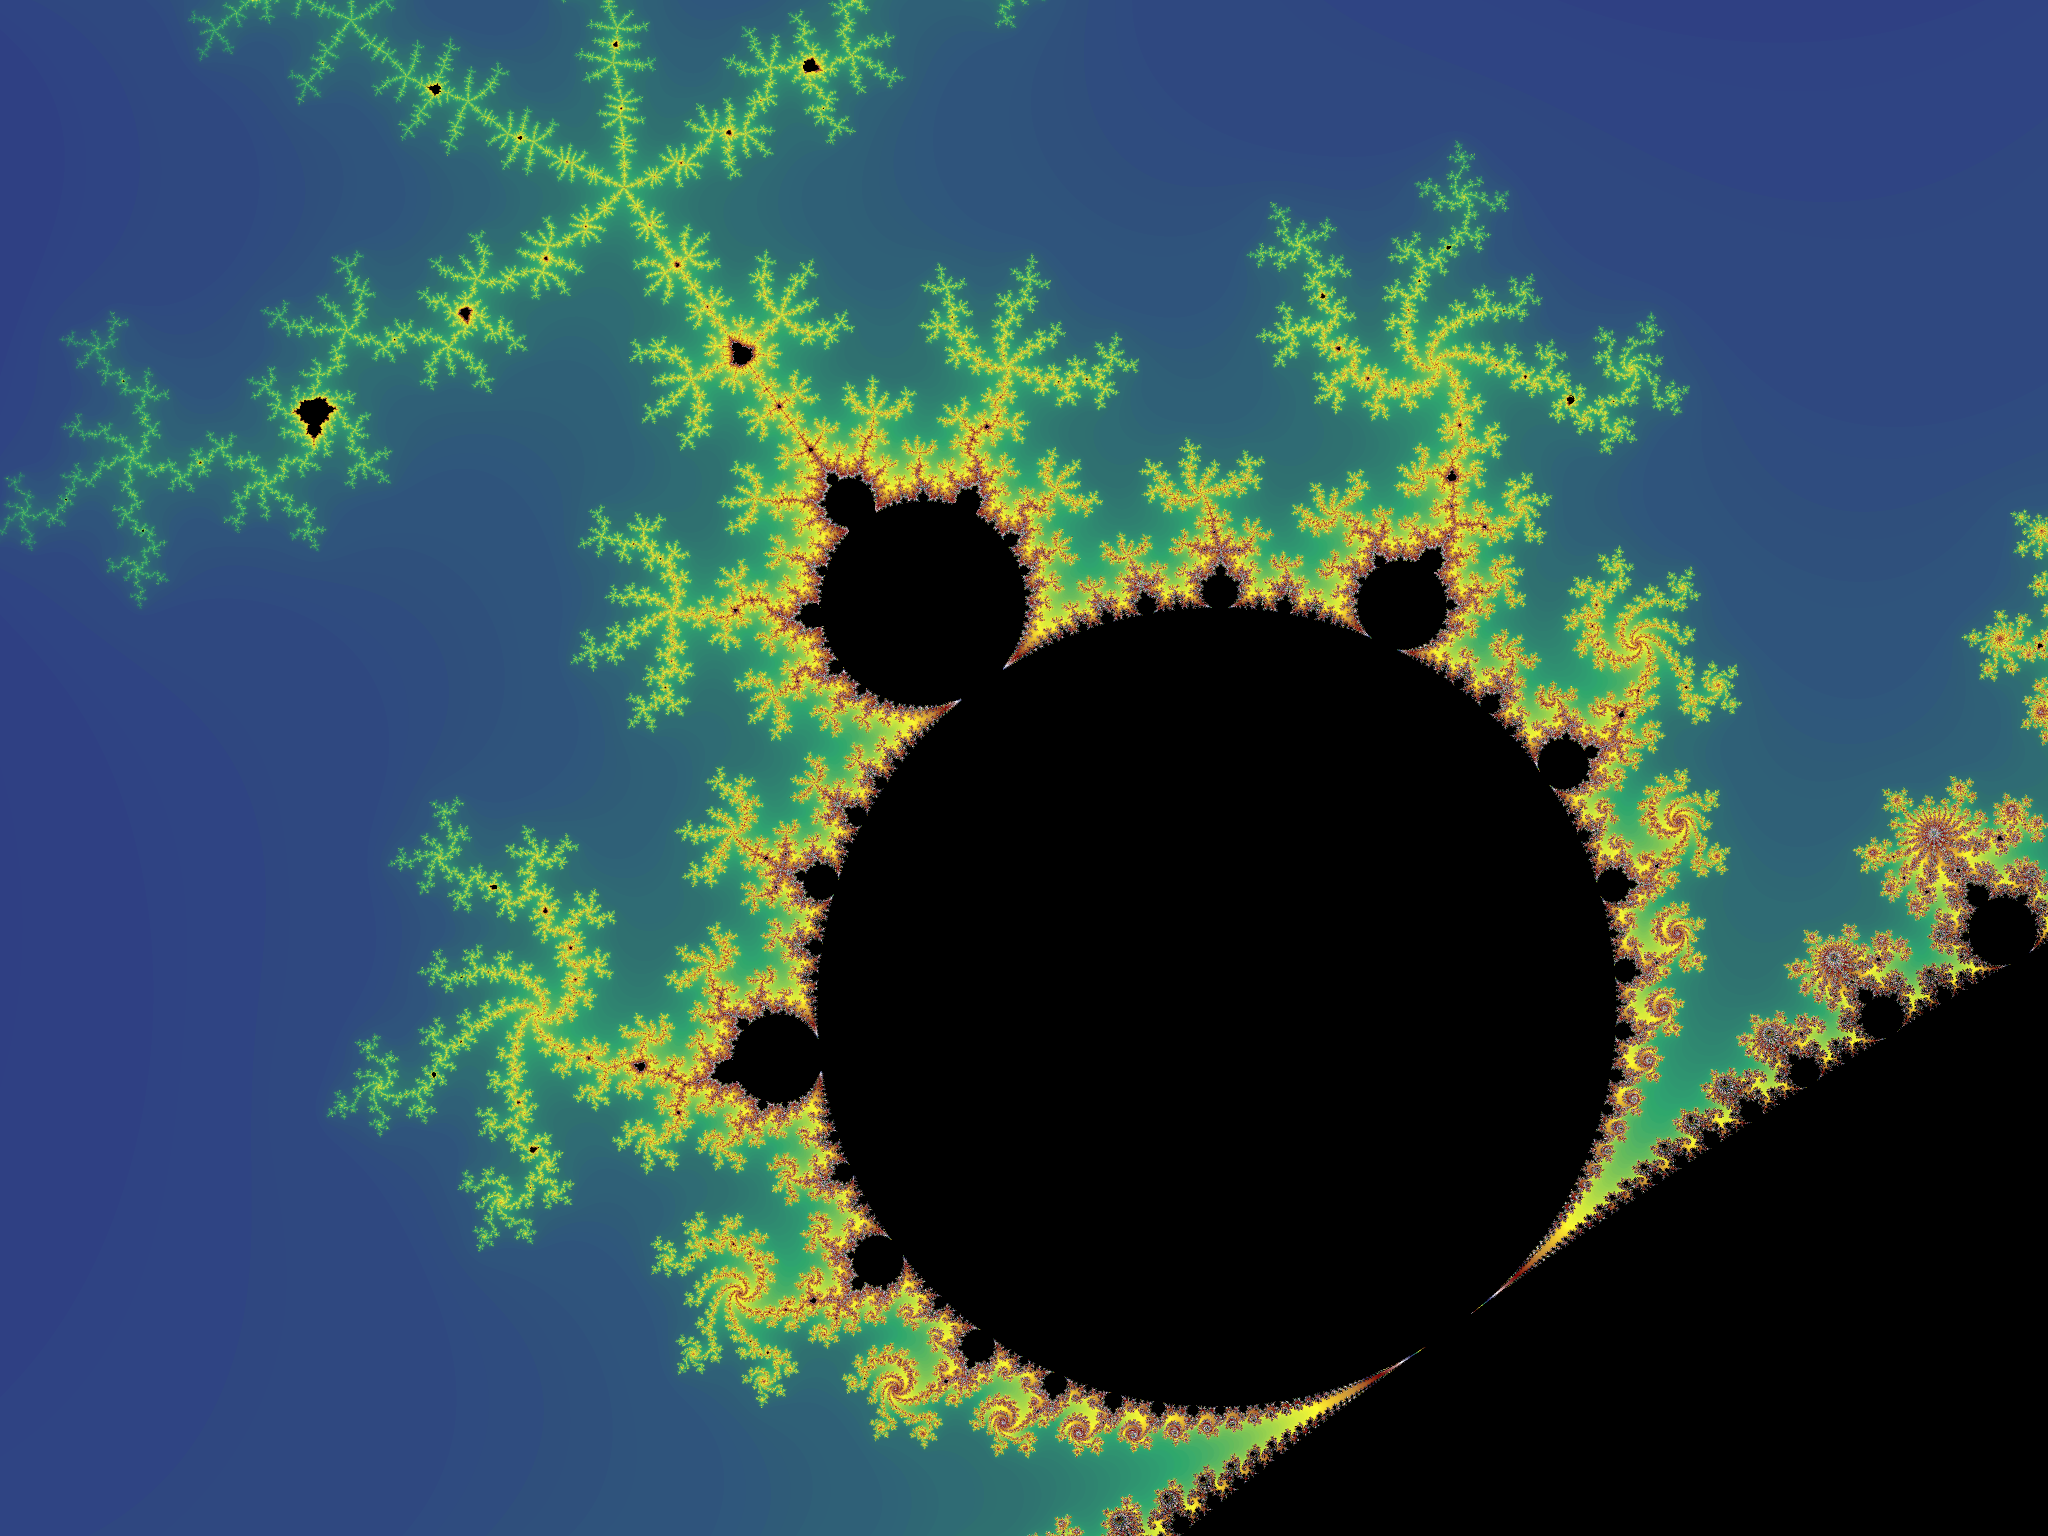
\includegraphics[width=\linewidth]{mandelbrot/1}
  \end{subfigure}
  \begin{subfigure}{0.49\linewidth}
    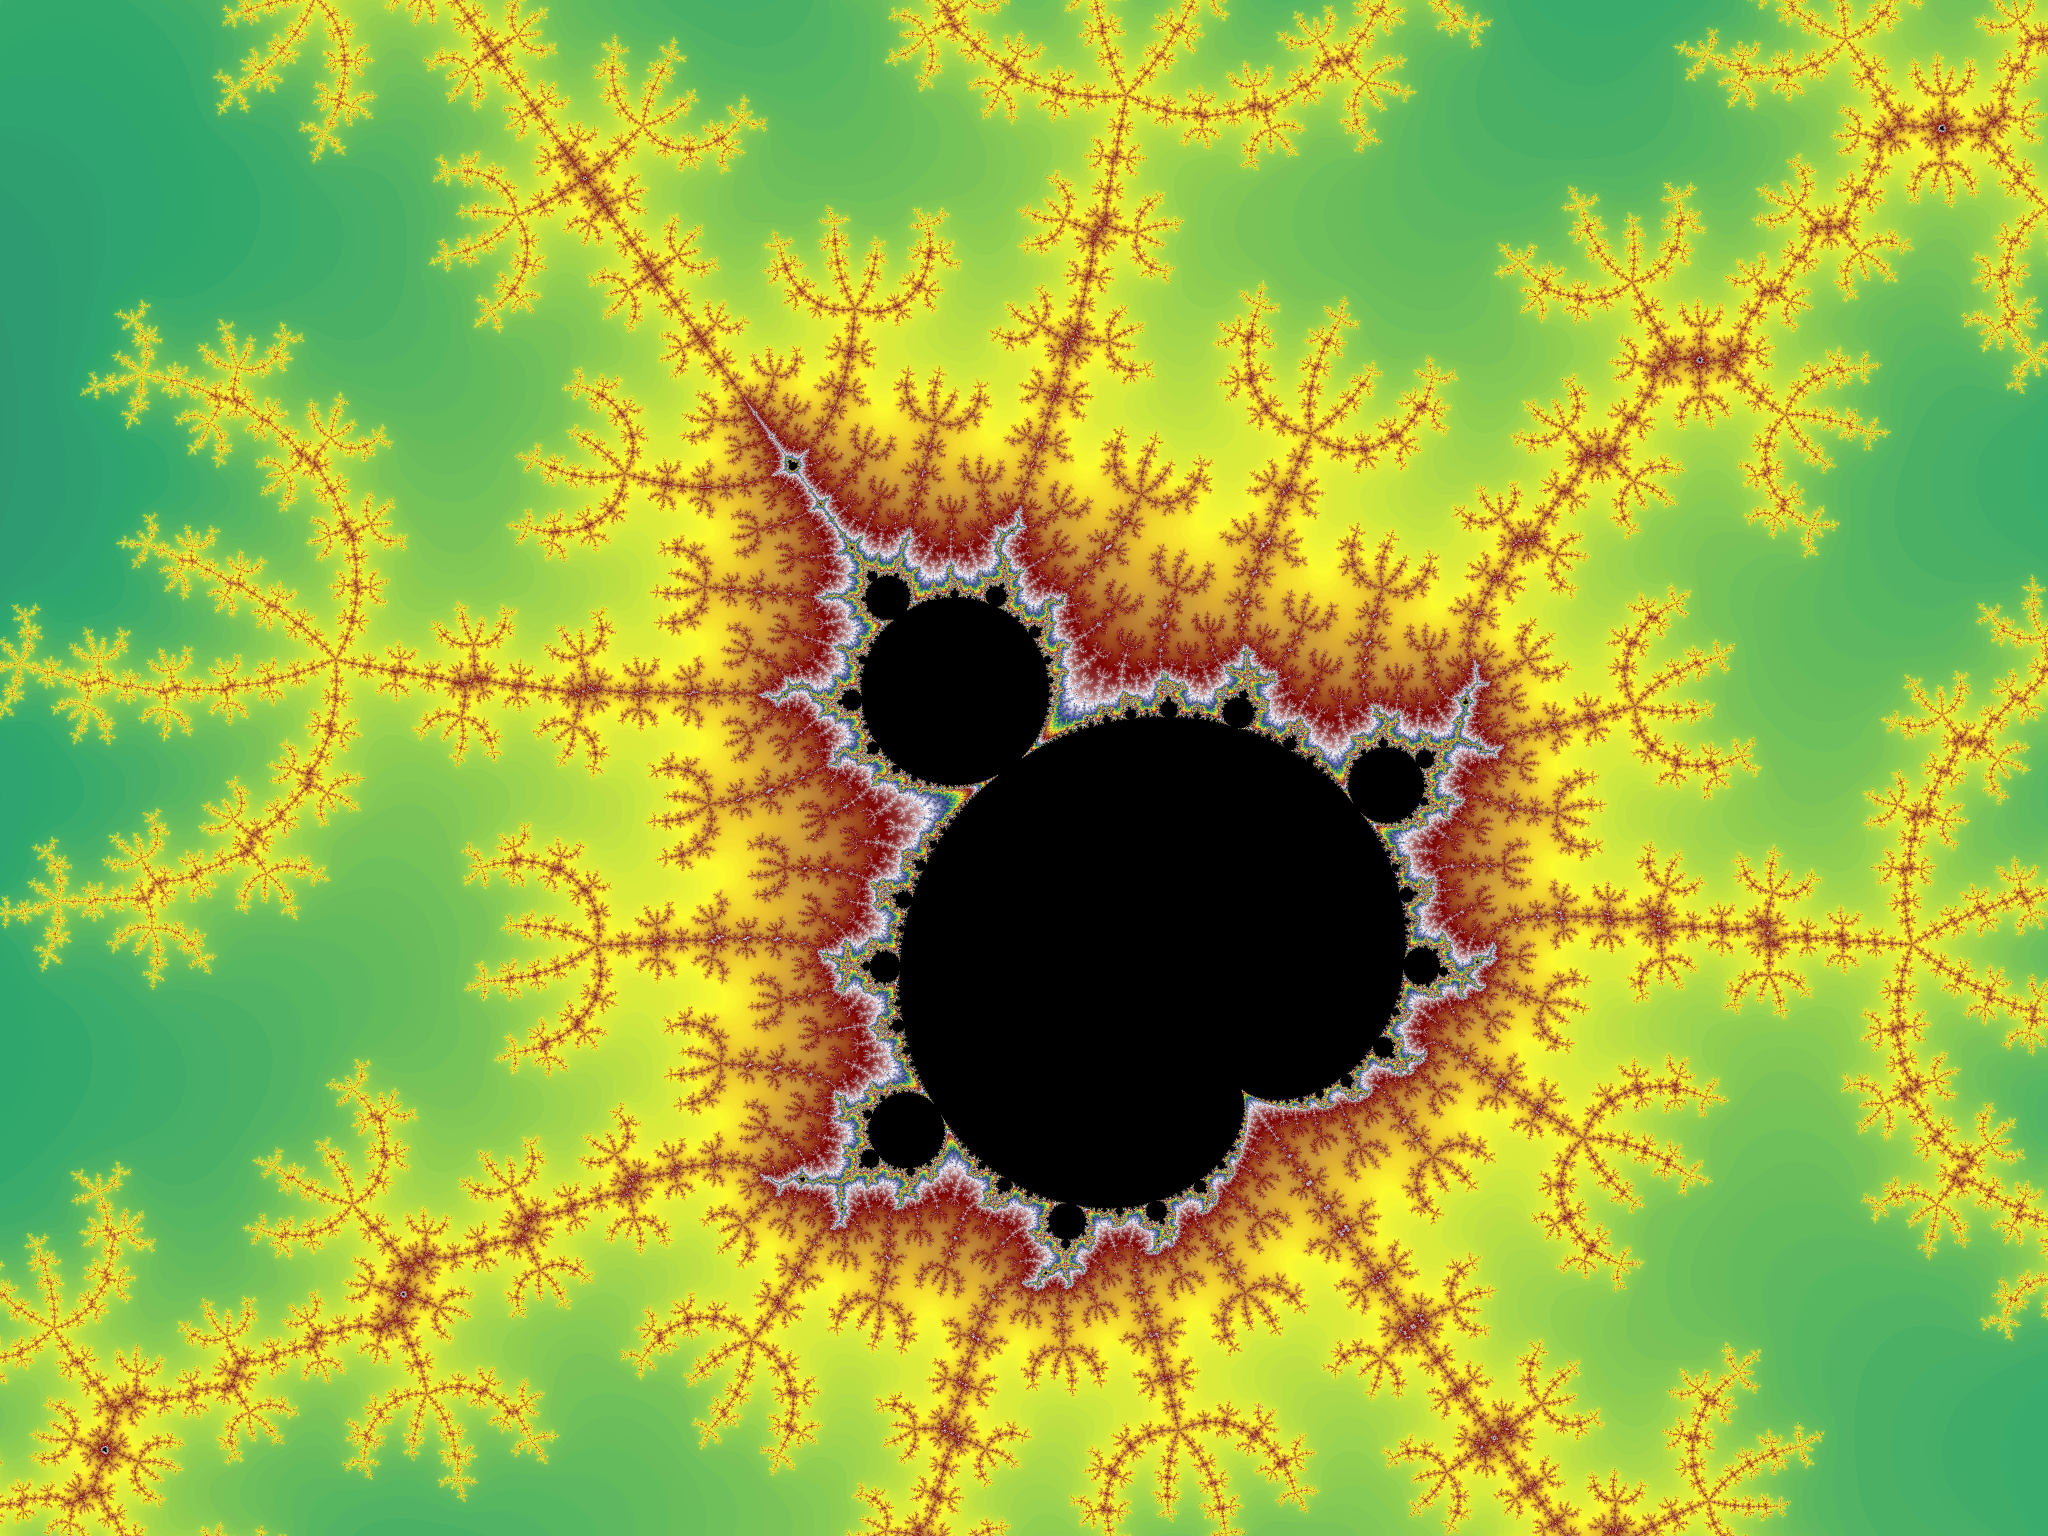
\includegraphics[width=\linewidth]{mandelbrot/2}
  \end{subfigure}
  \begin{subfigure}{0.49\linewidth}
    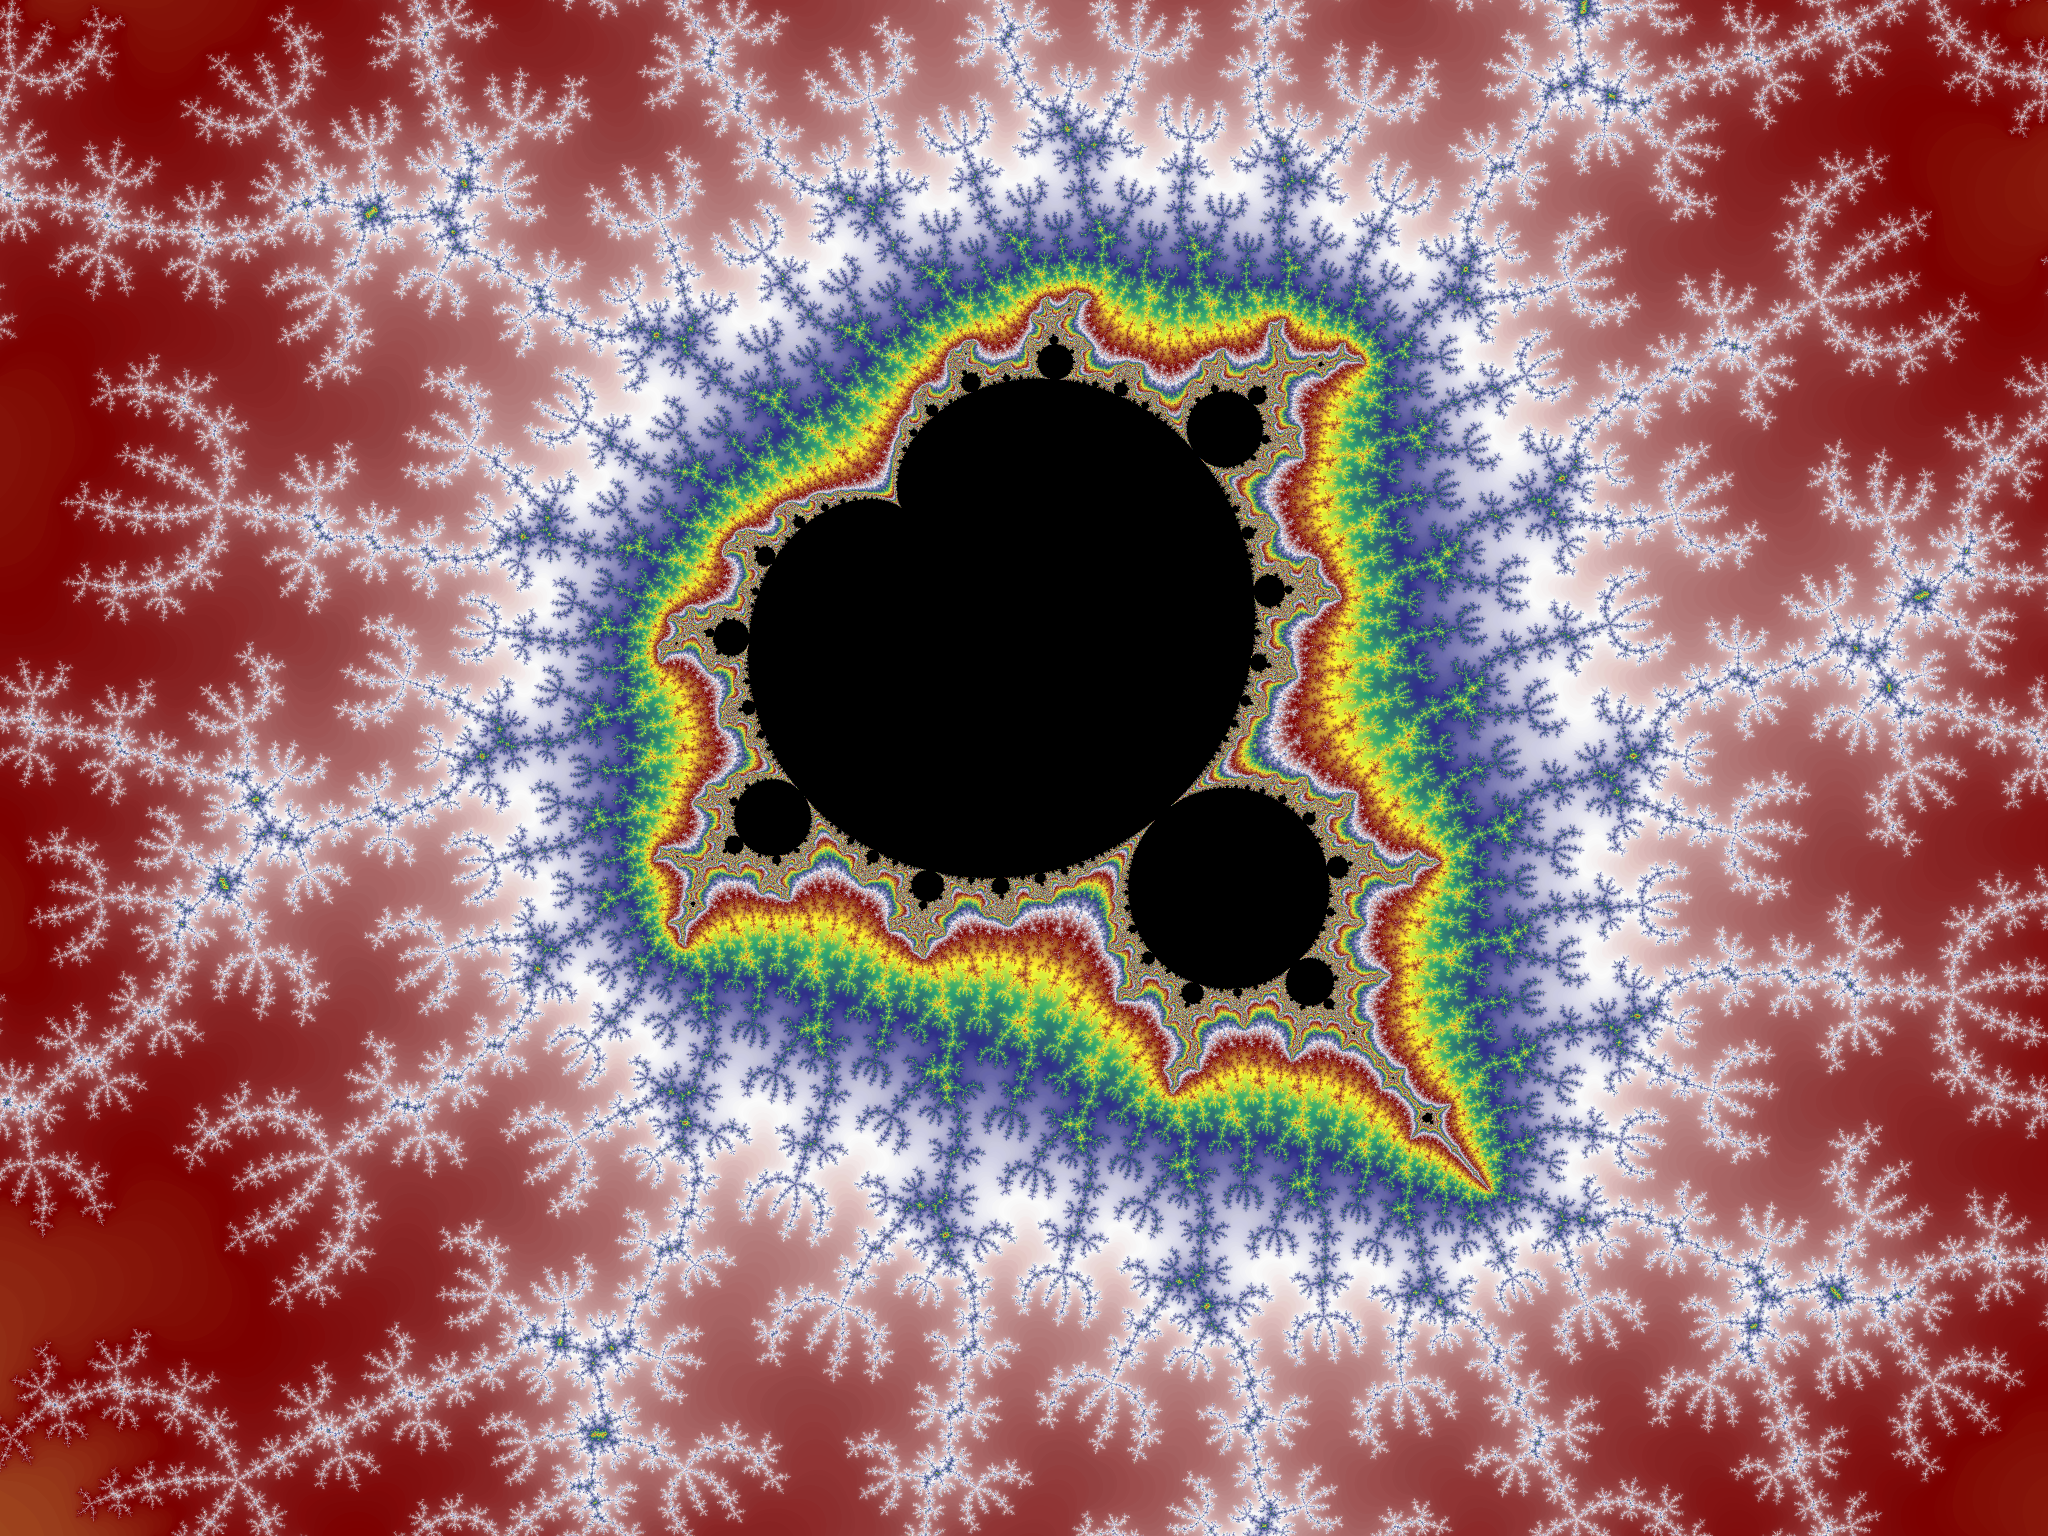
\includegraphics[width=\linewidth]{mandelbrot/3}
  \end{subfigure}
  \caption{Mandelbrot set which exhibits scale invariance as certain patterns
    repeat at different scales (above pictures showing different 'zoom' into the
    Mandelbrot set).}
  \label{fig:mandelbrot}
\end{figure}

\begin{figure}
  \centering
  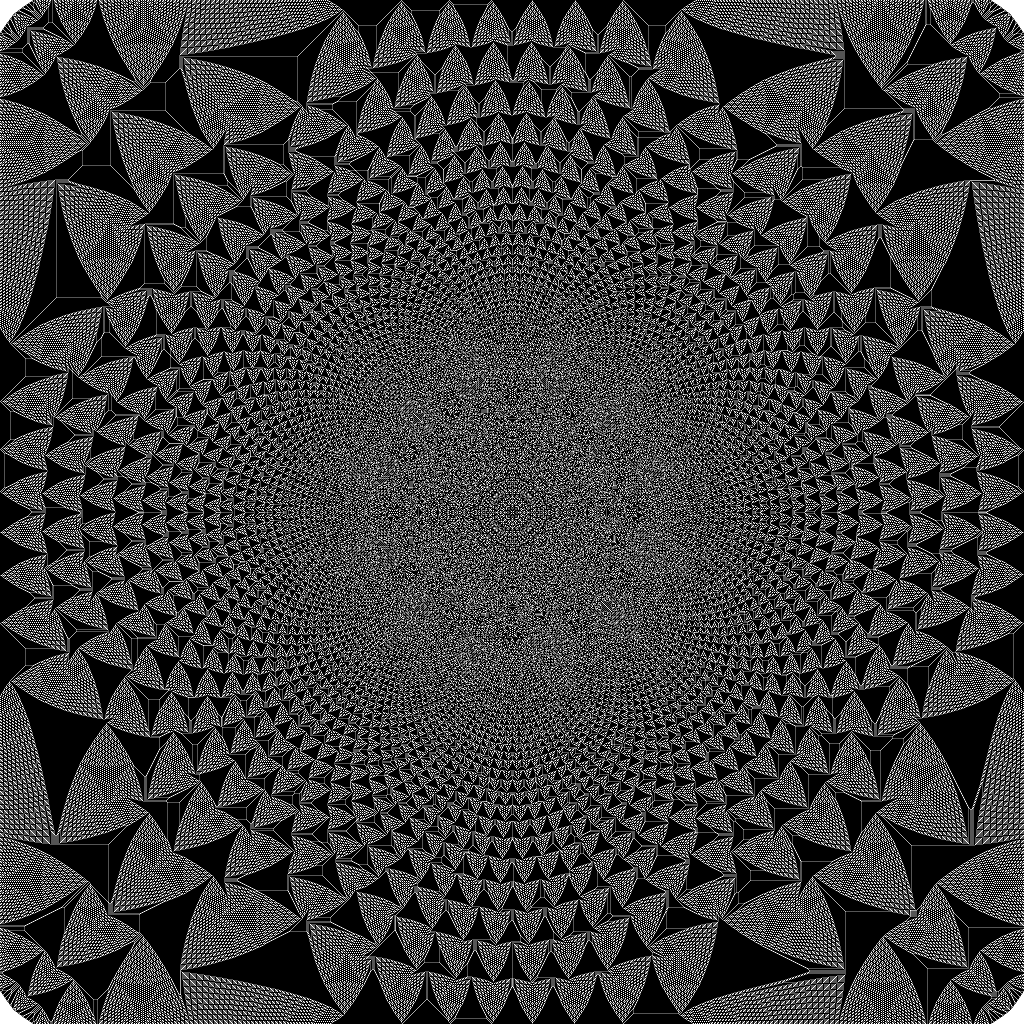
\includegraphics[width=0.8\linewidth]{sandpile}
  \caption{The \gls{BTW} sand pile exhibiting scale-invariant patterns.  In this
    sand pile, the sand was dropped continuously onto the centre.}
  \label{fig:sandpile}
\end{figure}

\begin{question}
  Why is it that a system exhibiting scale invariance will have phenomena
  which are described by a power law?
\end{question}

Self-organizing criticality as a framework has been used to study an
extraordinarily diverse range of systems.  It has been used to characterise,
analyze and predict earthquakes, financial markets, evolution and extinction
events, pulsar glitches, neuronal behaviour and much more.

\subsection{Non-equilibrium Statistics}
\label{subsec:non-equilibrium_statistics}

As discussed above, the systems we will be investigating have an enormous number
of degrees of freedom making it difficult to work with analytically and
impossible to solve the exact dynamics of the system.  In order to still get an
insight on the system, we must rely on statistical tools and in particular,
tools which work with non-equilibrium systems.

Non-equilibrium statistics underlies how we think about systems that display
self-organizing criticality and does so in a holistically.  When a system is
critical, microscopic phenomena (such as a local increases in stress) are not
responsible for the macroscopic observables of the system (such as an
earthquake's size, duration, area etc).  In particular, the proportions of large
and small events do not depend on the exact microscopic details of what is
happening.  Consequently, one cannot analyze the building blocks of a system in
order to explain the large scale phenomena.  In other words, a detailed
understanding of the microscopic interactions of the system do not translate
into system-level understanding.

\subsection{Aim}
\label{subsec:aim}

The primary aim of this lab will be to build a basic sand pile model and study
\gls{SOC} within this system and the associated non-Gaussian statistics.  The
basic model can subsequently be extended in any of a number of ways to replicate
more physically accurate systems or investigate how the system behaves under
different conditions.

\cleardoublepage
\section{Bak--Tang--Wiesenfeld Model}
\label{sec:bkw_model}

When modelling a complex system, it is often difficult (or impossible) to create
mathematical formalism that is both sufficiently realistic and
computationally/theoretically tractable.  As a result, researchers will consider
a simplified model that captures the important elements of the physical system
in question.  The \gls{BTW} model is an excellent example of a simplified
model which exhibits \gls{SOC}.

The \gls{BTW} model describes a (somewhat abstract) sand pile.  The grains of
sand are located on an \(N \times M\) lattice such that \(p_{t}(i, j)\) is the
number of grains located on site \((i, j)\) at time \(t\), where \(i \in [1,
  \dots, N]\), \(j \in [1, \dots, M]\) and \(t \inN^{0}\).  At each time step
\(t\), a new grain of sand is added to a random site in the lattice causing the
sand piles at each site to grow.

If an individual pile of sand reaches a height of 4 or more, then the pile
topples and distributes four grains of sand to its four immediate neighbours (we
are not considering diagonal neighbours):
\begin{equation}
  \label{eq:toppling_rule}
  \begin{aligned}
    p_{t}(i, j)       & = p_{t}(i, j) - 4,       \\
    p_{t}(i \pm 1, j) & = p_{t}(i \pm 1, j) + 1, \\
    p_{t}(i, j \pm 1) & = p_{t}(i, j \pm 1) + 1.
  \end{aligned}
\end{equation}
Note that this process is instantaneous and does not increment \(t\).
Furthermore, if the toppling happens on the edge of the lattice (i.e.~\(i \in
\{1, N\}\) and/or \(j \in \{1, M\}\)), the grains that would topple to a site
off the table are deleted from the system.

\begin{question}
  In what ways does the \gls{BTW} model satisfy the properties required for a
  system to exhibit \gls{SOC}?
\end{question}

\begin{question}
  Why is it important for the table to have finite boundaries?

  What if we had an infinite lattice, but dropped the sand on only a (finite)
  subset of the lattice?
\end{question}

If the lattice begins with no sand at all, we might expect the sand to just
accumulate to begin with as very few grains of sand will topple off the edge.
Eventually though, the slow addition of sand should balance out with those
grains of sand toppling off the edge of the grid.

\begin{question}
  We can define the average height of each pile to be:
  \begin{equation}
    \label{eq:average_height}
    \angles{p_{t}} \defeq \frac{1}{N M} \sum_{i, j} p_{t}(i, j).
  \end{equation}
  Without simulating anything, what might you expect this to be once the system
  has reached a steady state (if it ever does so)?  Compare your initial
  expectation to what your simulation does.
\end{question}

\begin{question}
  Explain the difference between: a steady state, a statistically stationary
  state, and an equilibrium state.

  Do you expect the \gls{BTW} model reach an equilibrium state or statistically
  stationary state?  In terms of system observables, how might we characterize
  this state?
\end{question}

The addition of a grain of sand to the lattice has a chance of creating an
unstable site which topples; but the toppling in turn can create further
unstable sites which will subsequently topple.  As a result, the addition of a
single grain of sand can create a chain of toppling which we call an
\emph{avalanche} as depicted in \cref{fig:avalanche}.  It will be these
avalanches that we will be most interested in.  In particular, we will consider
the following properties:
\begin{description}
  \item[Topples] The number of topples required to take the grid from its initial
        unstable configuration to a stable one;
  \item[Area] The number of unique sites which have been toppled;
  \item[Loss] The number of grains of sand which are toppled off the lattice; and,
  \item[Length] A \enquote{length} which characterizes the avalanche.
\end{description}

Note that we are purposefully leaving the \emph{length} definition quite vague.
You'll have to decide where from and to this length is defined, and which metric
to use (such as the \(L^{1}\)-norm or \(L^{2}\)-norm, a.k.a.~Manhattan distance
and Euclidean distance respectively).  Don't forget to justify your choice.

\begin{figure}
  \centering
  \renewcommand{\arraystretch}{1.2}
  \pgfplotstabletypeset{
    1 3 3
    2 4 2
    2 1 1
  }
  \(\rightarrow\)
  \pgfplotstabletypeset{
    1 4 3
    3 0 3
    2 2 1
  }
  \(\rightarrow\)
  \pgfplotstabletypeset{
    2 0 4
    3 1 3
    2 2 1
  }
  \(\rightarrow\)
  \pgfplotstabletypeset{
    2 1 0
    3 1 4
    2 2 1
  }
  \(\rightarrow\)
  \pgfplotstabletypeset{
    2 1 1
    3 2 0
    2 2 2
  }
  \caption{An example of a simple avalanche taking place on a \(3 \times 3\)
    grid.}
  \label{fig:avalanche}
\end{figure}

\begin{question}
  Is there a difference between sampling a system over time and sampling an
  ensemble of systems?  If so, under what circumstances?

  Hint: Look up the property of \emph{ergodicity} and argue whether or not you
  believe the \gls{BTW} model is ergodic.
\end{question}

\begin{question}
  Record the frequency with which avalanches have a specific number of topples,
  area, loss and length.  What kind of distribution do you get for each?

  If possible, can you find a fit for the distribution?  (E.g.~for a Gaussian,
  find the mean and width of the distribution; for a power law, find the
  exponent.)
\end{question}

\begin{question}
  Do you expect any correlation between the four properties we are recording for
  the avalanche?  Justify why/why not, then verify this with your simulation.
\end{question}

\subsection{Abelian Property}
\label{subsec:abelian_property}

Although the \gls{BTW} model is a model of \enquote{sand piles}, it is extremely
unrealistic---after all, sand piles aren't formed on a lattice and even if they
were, a site wouldn't go from four grains of sand to none from toppling on its
neighbours.  Nevertheless, it exhibits an extremely useful mathematical property
when it comes to analysing its behaviour: the topplings are Abelian.  In other
words, it doesn't matter in which order we execute each toppling, the end result
is the same.

To give a concrete example, consider the following start to an avalanche:
\begin{center}
  \Large
  \renewcommand{\arraystretch}{1.2}
  \pgfplotstableset{
    every head row/.style={output empty row},
    color cells={min=0, max=5},
  }
  \pgfplotstabletypeset{
    2 3 1
    1 4 0
    2 3 2
  }
  \(\rightarrow\)
  \pgfplotstabletypeset{
    2 4 1
    2 0 1
    2 4 2
  }.
\end{center}
There are now two unstable sites, \((1, 2)\) and \((3, 2)\).  If the model were
not Abelian, we would need to keep track of the order in which sites are toppled
and make sure that we topple the correct next unstable site; however as the
\gls{BTW} sand pile model is Abelian, we can do this in whatever order we wish
and arrive at the same result thereby greatly simplifying the computational
complexity of avalanches.

You might take it for granted that the \gls{BTW} model is Abelian, but this can
be fairly easily shown rigorously.  To begin with, we can consider the lattice
of sand piles to be \(L\) which is a finite subset of \(\bbZ^{d}\) where \(d\)
is the dimensionality of the lattice.\footnote{Although we will only be
  considering the case where \(d = 2\), it is no more difficult to show that the
  \gls{BTW} model is Abelian in arbitrary (finite) dimensions.}  For any site
\(\vt x \in L\), the number of grains of at each point of the lattice is given
by the function\footnote{For the sake of clarity, we are dropping the subscript
  \(t\) as we are dealing only with the toppling of sand within an avalanche
  during which \(t\) remains fixed.}
\begin{equation}
  p : L \to \bbN^{0}.
\end{equation}
A stable configuration corresponds to the scenario where \(p(\vt x) < k\) for
all \(\vt x \in L\) while an unstable one has at least one site \(\vt x \in L\)
where \(p(\vt x) \geq k\) where \(k\) defines is the stability threshold.

From an unstable configuration \(p\), we must introduce a way to describe the
toppling; for this, we introduce the toppling matrix \(\Delta(\vt x, \vt
y)\).  This stabilizes an unstable site \(\vt x\) in the configuration \(p\) by
redistributing the sand to site \(\vt y\).  The toppling matrix must satisfy the
following conditions:
\begin{subequations}
  \label{eq:toppling_matrix_conditions}
  \begin{align}
    \forall \vt x, \vt y \in L \text{ where } \vt x \neq \vt y,
     & \quad \Delta(\vt x, \vt y) = \Delta(\vt y, \vt x) \geq 0, \\
    \forall x \in L,
     & \quad \Delta(\vt x, \vt x) < 0,                           \\
    \forall x \in L,
     & \quad \sum_{\vt y \in L} \Delta(\vt x, \vt y) \leq 0,     \\
     & \quad \sum_{\vt x, \vt y \in L} \Delta(\vt x, \vt y) < 0.
  \end{align}
\end{subequations}

\begin{question}
  For each condition in \cref{eq:toppling_matrix_conditions}, explain the
  significance and justify its necessity.
\end{question}

The actual definition of the toppling matrix in the \gls{BTW} model is:
\begin{equation}
  \label{eq:btw_toppling_matrix}
  \Delta(\vt x, \vt y) =
  \begin{cases}
    -2d & \vt x = \vt y                               \\
    1   & \vt x, \vt y \text{ are nearest neighbours} \\
    0   & \text{Otherwise}
  \end{cases}.
\end{equation}
\begin{question}
  Explain and justify the definition of the toppling matrix in the \gls{BTW}
  model and verify that it satisfies all the conditions set out in
  \cref{eq:toppling_matrix_conditions}.  What is the stability threshold \(k\)?
\end{question}

Given the definition of the toppling matrix, it is now possible to define the
toppling operator \(T_{\vt x}\) which maps a configuration \(p\) to a new
configuration \(p'\):
\begin{equation}
  \label{eq:toppling_operator}
  (T_{\vt x} p)(\vt y) \defeq
  \begin{cases}
    p(\vt y) + \Delta(\vt x, \vt y) & p(\vt x) \geq \Delta(\vt x, \vt x) \\
    p(\vt y)                        & \text{Otherwise}
  \end{cases}.
\end{equation}

\begin{question}
  Show that \(T_{\vt x}\) and \(T_{\vt x'}\) commute for unstable
  configurations.
\end{question}

In general, multiple topplings are required in order to stabilize a
configuration \(p\) and we can introduce a stabilization operator which maps an
unstable configuration to a stable configuration
\begin{equation}
  \bbT : U_{L} \to S_{L}
\end{equation}
where \(U_{L}\) is the space of all possible height configurations and \(S_{L}
\subset U_{L}\) is the subset of stable height configurations.  To give a
concrete example, the stabilization operator for \cref{fig:avalanche} consists
of four topplings:
\begin{equation}
  p' = \bbT p = T_{(2,3)} T_{(1,3)} T_{(1,2)} T_{(2,2)} p.
\end{equation}
Thus we see that a stabilization operator can be represented as
\begin{equation}
  \bbT = \prod_{i=1}^{N} T_{\vt x_{i}}
\end{equation}
where \(N\) is the number of instabilities through an avalanche.

\begin{question}
  Show that \(\bbT\) is well defined.  In other words, show that given some
  unstable configuration \(p\), \(p' = \bbT p\) is unique (you can't end with
  two different stable configurations).  This is equivalent to the sequence of
  \(T_{\vt x_{i}}\) required is unique up to re-ordering.

  Hint: Read the original papers for hints as to how this can be done.
\end{question}

\section{Extending the \gls{BTW} Model}
\label{sec:extending_the_btw_model}

The \gls{BTW} model is clearly unrealistic; however, you have just seen that it
still exhibits very interesting statistics.  You can now extend this model in
any of a number of ways.  Irrespective of which extension(s) you choose,
remember to make predictions as to what you expect and then test these
predictions with your simulation.  You should also compare your extension to the
baseline \gls{BTW} model: in what ways is it similar and in what ways does it
differ?

A few extensions you may consider (and combine or extend as your please):
\begin{enumerate}
  \item Change the toppling so that it depends on the gradient: if a site has
        \(k\) more grains of sand than its neighbour it is unstable and it drops \(1\)
        grain of sand onto this neighbour and repeat until it is stabilized.
  \item Change the toppling to be random: instead of redistributing the four
        grains of sand to all four neighbours, it selects one of the four neighbours
        at random for each grain of sand.  What about adjusting the probability to
        drop to a neighbour based on the height difference?
  \item Change the boundary conditions:
        \begin{enumerate}
          \item Make the toppling \enquote{wrap around} in \(x\) (like a cylinder) so
                that grains of sand can only drop off the top or bottom of the grid.
          \item What happens if grains of sand can't topple off the edge, but instead
                there is a hole in the centre of the grid (imagine a kind of hourglass).
        \end{enumerate}
  \item Change how fast grains of sands are added to the grid.  Instead of adding
        1 grain of sand at a time, add 2, or 3, or \(n\).  Do you add each of these
        grains to different sites or the same?
  \item Change how you are adding grains of sand.  Instead of being uniformly
        random on the grid, what if grains of sand were only dropped on a small subset
        of the grid, or followed a different distribution (such as a Gaussian centred
        on the middle of the grid).
  \item Make the avalanche happen really slowly so that the toppling rule,
        \cref{eq:toppling_rule}, becomes:
        \begin{equation}
          \begin{aligned}
            p_{t+1}(i, j)       & = p_{t}(i, j) - 4,       \\
            p_{t+1}(i \pm 1, j) & = p_{t}(i \pm 1, j) + 1, \\
            p_{t+1}(i, j \pm 1) & = p_{t}(i, j \pm 1) + 1.
          \end{aligned}
        \end{equation}
        Perhaps you don't want to increase the timestep every topple, but every
        \(n\)th topple.
  \item Instead of a rectangular lattice, change it to a hexagonal lattice (have a
        look at \emph{hexagonal coordinate systems}).
  \item Change the toppling rule so that instead of dropping to the 4 directly
        adjacent sites, it drops to the 8 surrounding sites.  Or maybe change it so
        that it drops to all sites with a radius of 2 of the initial site.
  \item Add a force that will push grains of sand in a particular direction
        (such as wind, or if the grid was sloped).
\end{enumerate}

\cleardoublepage
\printbibliography

\end{document}